\documentclass[conference]{IEEEtran}
\usepackage{cite}
\usepackage{amsmath,amssymb,amsfonts}
\usepackage{algorithmic}
\usepackage{graphicx}
\usepackage{textcomp}
\usepackage{comment}
\renewcommand{\refname}{Referencias}
\renewcommand{\tablename}{TABLA}


\def\BibTeX{{\rm B\kern-.05em{\sc i\kern-.025em b}\kern-.08em
    T\kern-.1667em\lower.7ex\hbox{E}\kern-.125emX}}
\begin{document}
\title{Predicción de la posibilidad de muerte del paciente de infarto de miocardio utilizando Bosques Aleatorios}

\author{\IEEEauthorblockN{Juan Acostupa}
\IEEEauthorblockA{\textit{Dpto. de Ing. Informática PUCP} \\
Lima, Perú\\
a20244906@pucp.edu.pe}
\and
\IEEEauthorblockN{Breno Muñoz}
\IEEEauthorblockA{\textit{Dpto. de Ing. Informática PUCP} \\
Lima, Perú\\
a20162955@pucp.edu.pe}
\and
\IEEEauthorblockN{Ronny Huerta}
\IEEEauthorblockA{\textit{Dpto. de Ing. Informática PUCP} \\
Lima, Perú \\
a20184255@pucp.edu.pe}
}

\maketitle

\section{\textbf{Introducción}}
El ataque al miocardio es una de las complicaciones de salud que causan más muertes a nivel mundial. En el Perú, más de 4 mil personas mueren al año debido a esta emergencia médica \cite{b2}. Las causas de esta condición son conocidas: enfermedad de las arterias coronarias, acumulación de colesterol, artereoesclerosis, coágulos de sangre en las arterias, atero-trombosis, edad, sedentarismo y una alimentación desbalanceada. Sin embargo, es una enfermedad que puede ocasionar complicaciones diversas al paciente, entre las cuales la más letal es la muerte. Si bien no se conocen relaciones causa-efecto claras para la aparición de todas estas complicaciones, existen estudios que han hallado patrones entre las condiciones fisiológicas que manifiesta el paciente durante la aparición de la enfermedad, los cuales pueden aprovecharse con modelos de aprendizaje automático para predecir si el paciente de infarto al miocardio puede sufrir alguna de estas complicaciones\cite{b1}. En este sentido, el presente estudio se focaliza en la predicción de la complicación más letal: la muerte del paciente. Esto con el fin de que el personal asistencial pueda decidir un curso de acción a tiempo. 

A continuación, se establece el siguiente orden de secciones para este artículo. En primer lugar, se describe una introducción general a la problemática (\textbf{Sección I}) junto con el objetivo principal a abordar en el presente trabajo; en la segunda parte (\textbf{Sección II}) se hace una breve síntesis del estado del arte con artículos científicos usando los mismos datos del presente proyecto y con otros diferentes pero con alternativas de solución en relación al problema mencionado; en la tercera parte (\textbf{Sección III}) se explica sobre el diseño del experimento, en el cual se realiza una descripción del conjunto de datos y la metodología a usar para el abordaje del presente proyecto.

\section{\textbf{Estado del arte}}
Existen múltiples trabajos que tratan diferentes aspectos relacionados a la utilización de algoritmos de aprendizaje automático y la importancia del rol que juegan estos métodos en la mejora del diagnóstico y prevención de complicaciones. \textit{Quer et. al.} \cite{e1} hace un énfasis especial en el rol que desempeña el personal médico, en especial los cardiólogos. Asimismo, \textit{Van den Eynde et. al.} \cite{e2} hace mención de un número de ejemplos exitosos de técnicas de inteligencia artificial para aplicaciones de cardiología clínica; mientras que \textit{Sevakula et. al.} \cite{e3} hace un estudio sobre nuevos casos que se le pueden dar a estas técnicas, además de las limitaciones que estas tienen. Finalmente, \textit{Benzakour et. al.} \cite{zz} hace un estudio extenso de los conjuntos de datos publicados sobre distintas enfermedades cardiovasculares con el cual identificó 39 conjuntos de datos. Uno de estos es el "Myocardial Infarction Complications Database", el mismo que se ha seleccionado como objeto de estudio del presente trabajo.

El dataset Myocardial Infarction Complications Database se ha utilizado previamente para predecir complicaciones en pacientes que han sufrido infarto del miocardio. A continuación se resumen las metodologías respecto del tratamiento de los datos y los modelos de clasificación sobre estos mismos datos y sobre otras bases de datos \cite{bp}. 

\subsubsection{\textbf{Preprocesamiento}}
Respecto del preprocesamiento de los datos, algunos autores coinciden en tratar los datos faltantes eliminando aquellas variables cuyos faltos exceden un límite porcentual máximo. Otros autores optan por reemplazar los valores faltantes con el valor constante de "-1" con el fin de poder identificar claramente en dónde suceden valores faltantes al momento de explicar las salidas de modelos de tipo árbol\cite{bref}. En cambio, otros utilizan técnicas de reducción de la dimensionalidad\cite{bp} como el Análisis de Componentes Principales (PCA) y el catPCA. Teóricamente, este último está pensado para mantener la máxima correlación entre las variables cuando se tienen salidas con datos de tipo categórico \cite{b1}. También,  autores han tomado la alternativa de utilizar técnicas más sofisticadas como la Coincidencia de Medias Predictiva (PMM) para intentar imputar valores nulos \cite{ll}. También, se observa que se ha intentado abordar el desbalance de clases utilizando métodos tanto de sobre o sub muestreo como también métricas sensibles a la clasificación de la clase minoritaria (por ejemplo, la puntuación F1 o el área bajo la curva ROC)\cite{by}\cite{ll}

\subsubsection{\textbf{Clasificadores}}
 En esta categoría se han implementado modelos como Regresión Logística\cite{bx}\cite{bz}, Redes Neuronales \cite{bx}\cite{bz}\cite{ll}\cite{bp}, XGBOOST\cite{bz}\cite{bp}, Máquina de Vectores de Soporte (SVM)\cite{bz}, Bosques Aleatorios\cite{bz} y k-Vecindarios Más Cercanos\cite{b?}\cite{by}. Esto puede deberse a que tales modelos son adecuados para la clasificación de variables del tipo categórico. En general, se observa un éxito entre moderado y alto el cual puede depender de las variables que se eligen para realizar la predicción, donde individualmente se ha logrado sobrepasar métricas en más de 91\%. En este aspecto, destacan la aplicaciones de modelos basados en árboles de decisión debido a la relación entre su simpleza y el desempeño que se obtiene de estos.

\section{\textbf{Diseño del Experimento}}
\subsection{\textbf{Descripción del conjunto de datos}}\label{EDA}
El conjunto de datos contiene información de las condiciones fisiológicas de los pacientes que han sufrido un infarto al miocardio y complicaciones asociadas a esta afección. De acuerdo a \cite{b1}, este conjunto de datos contiene registros recolectados por el Hospital Clínico Interdistrital de Krasnoyarsk, en Rusia, durante los años 1992-1995. 
\subsubsection{Número y Tipo de variables}\label{nvar}
El conjunto de datos consta de dos partes. La primera contiene variables que se pueden considerar "de entrenamiento", conformando un total de 110. Estas variables incluyen:
\begin{itemize}
    \item 78 variables binarias.
    \item 16 variables categóricas.
    \item 9 variables numéricas discretas.
    \item 7 variables numéricas contínuas.
\end{itemize}

Algunas de las características más relevantes contienen información demográfica, antecedentes médicos (arritmias, insuficiencias cardiacas, entre otros), factores de riesgo cardiovascular e información de los primeros días de seguimiento al paciente post-infarto.

La segunda parte del conjunto de datos consta de variables que contienen información de diferentes tipos de complicaciones relacionadas a infarto en el miocardio. Estas variables se pueden considerar como "objetivos", y son un total de 12, siendo estas:
\begin{itemize}
\item 11 variables binarias.
\item 1 variable categórica.
\end{itemize}

\subsubsection{\textbf{Número de muestras}}\label{nmue}
El conjunto de datos contiene un total de 1700 registros. No existe una separación entre conjunto de entrenamiento y conjunto de prueba, pero esta separación es necesaria para cumplir con el objetivo del presente análisis, por lo que se va a realizar siguiendo la estrategia utilizada en la sección de metodología.

\subsubsection{\textbf{Número de muestras por clase}}\label{nmue}
Este conjunto de datos contiene un total de 12 variables que se pueden considerar como objetivo, de las cuales 11 son binarias. La distribución de clases de cada una de estas variables binarias es:

\begin{table}[ht]
\centering
\caption{Número de muestras por variable binaria}
\begin{tabular}{l|r|r}
\textbf{Variable} & \textbf{Clase = 0} & \textbf{Clase = 1} \\
\hline
\rule{0pt}{3ex}
    FIBR\_PREDS & 1530 & 170 \\
    PREDS\_TAH & 1680 & 20 \\
    JELUD\_TAH & 1658 & 42 \\
    FIBR\_JELUD & 1629 & 71 \\
    A\_V\_BLOK & 1643 & 57 \\
    OTEK\_LANC & 1541 & 159 \\
    RAZRIV & 1646 & 54 \\
    DRESSLER & 1625 & 75 \\
    ZSN & 1306 & 394 \\
    REC\_IM & 1541 & 159 \\
    P\_IM\_STEN & 1552 & 148 \\
\end{tabular}
\label{tab:num_samples}
\end{table}

Mientras tanto, la variable categórica tiene la siguiente distribución:

\begin{table}[ht]
\centering
\caption{Distribución de clases de la variable categórica LET\_IS}
\begin{tabular}{c|c}

\textbf{Valor de LET\_IS} & \textbf{Frecuencia} \\
\hline
    \rule{0pt}{3ex}
    0 & 1429 \\
    1 & 110 \\
    3 & 54 \\
    7 & 27 \\
    6 & 27 \\
    4 & 23 \\
    2 & 18 \\
    5 & 12 \\

\end{tabular}
\label{tab:let_is_dist}
\end{table}

Por un lado, las variables de predicción del dataset sufren del problema del desbalance. Generalmente, se observa una proporción de alrededor 1 a 9 entre casos positivos y negativos (\textbf{Tablas \ref{tab:num_samples} y \ref{tab:let_is_dist}}), respectivamente. En base a esto, será necesario tomar en cuenta el problema de el desbalance de clases durante el entrenamiento para evitar el sesgo hacia la clase negativa. 

Por otro lado, las variables de entrada contienen una gran cantidad de valores faltantes. De las 110 variables de entrada, 11 de ellas presentan al menos 20\% de valores faltantes (\textbf{Tabla \ref{above_20_misssing_values_from_input}}).

\begin{table}[ht!]
\centering
\caption{Variables con más de 20\% de valores faltantes}
    \begin{tabular}{l|c}
    \textbf{Variable} & \textbf{Porcentaje de valores faltantes} \\
    \hline
    \rule{0pt}{3ex}
    IBS\_NASL     & 95.7 \\
    S\_AD\_KBRIG   & 63.2 \\
    D\_AD\_KBRIG   & 63.2 \\
    GIPO\_K       & 21.7 \\
    K\_BLOOD      & 21.8 \\
    GIPER\_NA     & 22.0 \\
    NA\_BLOOD     & 22.0 \\
    KFK\_BLOOD    & 99.7 \\
    NA\_KB        & 38.6 \\ 
    NOT\_NA\_KB    & 40.3 \\
    LID\_KB       & 39.8 \\
    \end{tabular}
\label{above_20_misssing_values_from_input}
\end{table}

\subsubsection{\textbf{Estadística descriptiva}}\label{edes}
Este conjunto de datos contiene información de 111 variables que brindan información de aspectos fisiológicos relacionados al paciente infartado durante su admisión y estancia  en el hospital. Para poder obtener información del conjunto de datos, se ha optado por utilizar un algoritmo de clustering sobre la base de correlaciones, con lo cual, se han agrupado las 111 variables en 5 categorías distintas. La \textbf{Figura \ref{fig:fig1}} muestra una representación visual del método de clustering basado en la correlación entre variables utilizado.

De acuerdo a las variables agrupadas en cada clúster, se puede interpretar a grandes razgos a cada cluster de la siguiente manera:

\begin{itemize}
    \item Clúster \#1: (38 variables) Características generales del paciente, antecedentes médicos, hallazgos electrocardiográficos y manejo inicial en la unidad de cuidados intensivos.
    \item Clúster \#2: (8 variables) Seguimiento de los síntomas y manejo del dolor en los primeros días de hospitalización.
    \item Cluster \#3: (34 variables) Factores de riesgo cardiovascular, hallazgos clínicos y de laboratorio al ingreso, y manejo terapéutico inicial. 
    \item Clúster \#4: (27 variables) Antecedentes de arritmias e insuficiencia cardíaca, y hallazgos electrocardiográficos y clínicos relacionados al ingreso.
    \item Clúster \#5: (4 variables) Niveles séricos de electrolitos clave (potasio y sodio).
\end{itemize}

\begin{figure}[htbp!]
  \centering
  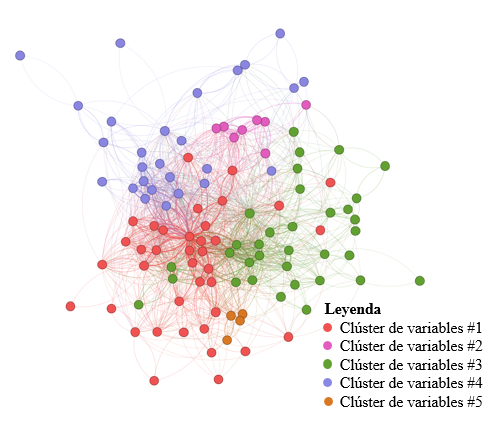
\includegraphics[width=8cm\textwidth]{mapa_correlaciones_con_leyenda.png} 
  \caption{Clustering de las 111 variables basado en correlaciones.}
  \label{fig:fig1}
\end{figure}

\subsection{\textbf{Metodología}}
El planteamiento del plan de acción está basado en tres aspectos de las características del dataset. A continuación se explica cada uno de ellos. 

En primer lugar, respecto de las variables de predicción, el dataset contiene once variables objetivo de naturaleza binaria y una variable categórica que puede tomar 7 categorías diferentes. Por ello, se puede tratar el problema tanto como uno de clasificación
con múltiples clases (multiclass) o múltiples etiquetas (multilabel). De acuerdo con otros trabajos realizados sobre el mismo dataset, se tomó la decisión de tratar el problema como uno de clasificación binaria. Así, el objetivo se convierte en crear un modelo que diferencie a los pacientes que tienen un desenlace letal ("LET\_IS" $\neq$ 1) de los pacientes que viven ("LET\_IS" = 1). En tal medida, las clasificaciones de esta naturaleza se pueden abordar con los siguientes modelos:

\begin{itemize}
    \item Regresión logística
    \item Árboles de decisión
    \item Máquinas de vectores de soporte
    \item Modelos de gradient boosting (LightGBM)
\end{itemize}
Dado el mayor éxito obtenido con modelos basados en árboles, se utilizará el modelo RandomForest que se ha estudiado en clase.

En segundo lugar, es evidente que las variables de predicción están fuertemente sesgadas hacia la clase negativa. Para abordar este problema se considera probar las siguientes técnicas: subsampleo, \textit{k-folds} con validación cruzada y técnicas de \textit{boosting} para árboles de decisión. Adicionalmente, por esta misma razón se entrenará los modelos con las métricas de AUC-PR y F1 con pesos como objetivo. Esto debido a que se caracterizan por ser sensibles a la clase minoritaria valorando el desempeño de los modelos tanto sobre la clase negativa como positiva\cite{b?}. 

En tercer lugar, es necesario abordar la gran cantidad de valores faltantes en las 111 variables mencionadas previamente. Al respecto, los autores consultados coinciden con eliminar las variables que presentan excesiva cantidad de faltos, cada uno por distintos criterios y/o reducirlos por medios de técnicas de reducción de la dimensionalidad. A criterio personal, se intentará conservar la mayor cantidad de información útil. Por ello, se procederá a reducir la dimensionalidad eliminando las variables que presenten nula correlación con la muerte del paciente y los valores nulos restantes serán reemplazados por un valor constante "-1". Como criterio de selección de características, se utilizará previamente un DecisionTreeClassifier para seleccionar las variables con una importancia mayor a 0.

Al final, se elegirá al mejor modelo  basado en la comparación de las métricas. En otras palabras, se probará distintos parámetros mediante una búsqueda en grilla o alguna herramienta como Optuna \cite{bopt} para hallar aquellos con mejor desempeño.

\section{\textbf{Experimentación y resultados}}
\subsection{\textbf{Línea base}}
Se ha tomado como referencia el trabajo desarrollado por Garcez, et. al. en \cite{bref}. En este trabajo, los autores seleccionaron 61 variables, las cuales fueron procesadas de la forma indicada en la publicación. A modo de resumen, el proceso de desarrollo del modelo en esta referencia sigue el siguiente proceso:

\begin{enumerate}
    \item Definición de target: Objetivo binario, paciente sobrevive o no (variable "LET IS" $\neq$ 0).
    \item Selección de variables.
    \begin{enumerate}
        \item Se eliminan columnas con más de 10\% de valores nulos.
        \item Se eliminan columnas con prevalencia de clase principal mayor al 95\%.
    \end{enumerate}
    \item Transformación de variables.
    \begin{enumerate}
        \item Se aplica One Hot Encoding para variables categóricas nominales.
        \item Se Escalan las variables entre 0 y 1 (MinMaxScaler).
    \end{enumerate}
    \item Imputación de valores nulos.
    \begin{enumerate}
        \item Variables categóricas con la moda.
        \item Variables numéricas con la mediana.
    \end{enumerate}
    \item Balanceo de datos: Undersampling al 50\%.
    \item Segunda selección de variables: Selección de las 50 variables con mayor correlación con el target.
    \item Entrenamiento del modelo.
\end{enumerate}

Los resultados obtenidos para distintas medidas de desempeño se muestran en la Tabla \ref{tab:base_performance}.

\begin{table}[h!]
\centering
\caption{Resultados de trabajo base}
\label{tab:base_performance}
\begin{tabular}{l|cccc}
\rule{0pt}{3ex}
Model & wF1 & wPrecision & wRecall & Accuracy \\
\hline
\rule{0pt}{3ex}
RandomForest & 0.900 & 0.899 & 0.903 & 0.903 \\
LightGBM & 0.912 & 0.914 & 0.918 & 0.918 \\
\rule{0pt}{3ex}
\end{tabular}
\end{table}

\subsection{\textbf{Resultados obtenidos}}
La propuesta desarrollada tomará como base el esquema de validación utilizado por Garcez, et. al. en \cite{bref}: Score promedio de un proceso de validación cruzada con 10 particiones. Los resultados obtenidos se muestran en la Tabla \ref{tab:resultados_modelos}. Asimismo, los parámetros del modelo con mejor desempeño se muestran en la \textbf{Figura \ref{modelo}}.

\begin{table}[h!]
\centering
\caption{Resultados del trabajo propuesto}
\begin{tabular}{l | llll}
\rule{0pt}{3ex}
Modelo & wF1 & wPrecision & wRecall & Accuracy \\
\hline
\rule{0pt}{3ex}
LogisticRegression & 0.88 & 0.893 & 0.896 & 0.896 \\
SVM & 0.893 & 0.910 & 0.909 & 0.909 \\
RandomForest & 0.906 & 0.921 & 0.919 & 0.919 \\
\rule{0pt}{3ex}
\end{tabular}
\label{tab:resultados_modelos}
\end{table}

Se ha logrado obtener resultados similares a los alcanzados por el trabajo que se ha tomado como referencia. En algunos casos, nuestro modelo ha superado , ligeramente y en algunas métricas, los resultados obtenidos por Garcez et. al., siendo el modelo RandomForest el que ha alcanzado el mejor rendimiento. 

\begin{figure}[htbp!]
  \centering
  \includegraphics[width=8cm\textwidth]{modelo.png} 
  \caption{Parámetros del modelo con mejor desempeño: RandomForest}
  \label{modelo}
\end{figure}


\section{\textbf{Discusión}}
En general, los modelos desarrollados han logrado igualar o mejorar el desempeño de las publicaciones revisadas en cuanto a predicción de la muerte del paciente se refiere. Esto es consistente en las distintas métricas evaluadas para los tres modelos evaluados en las tablas \ref{tab:base_performance} y \ref{tab:resultados_modelos}. 

De la misma manera, se observa que el problema del desbalance de clases no ha tenido impacto al momento de clasificar los 271 casos positivos para el deceso del paciente frente a los 1429 negativos. Esto se puede concluir del hecho de que tanto el Accuracy, como métrica susceptible de sesgo, como las métrica F1 y la sensibilidad y especificidad se mantienen con valores altos. En este sentido, se puede decir que la búsqueda en grilla junto con los métodos de validación cruzada han tenido el efecto deseado para la clasificación de los datos y por tanto se ha logrado abordar el problema del desbalance de las clases.

Finalmente, dado que el mejor modelo corresponde a uno basado en árboles de decisión, se procede a utilizar el método SHAP para explorar la importancia de las variables. El gráfico de resumen de SHAP es útil para identificar rápidamente cuáles variables de entrada tienen más impacto en el modelo y cómo sus afectan las predicciones o negativas o positivas. El gráfico SHAP está disponible en la \textbf{Figura \ref{shap}}. De acuerdo con esto, los resultados de este gráfico se pueden tomar como sugerencia para saber a cuáles condiciones clínicas del paciente infartado se les deben prestar mayor atención para identificar qué pacientes sufren mayor riesgo de morir. 

\begin{figure}[htbp!]
  \centering
  \includegraphics[width=8cm\textwidth]{shap_values.png} 
  \caption{Condiciones más importantes para la muerte del paciente según el método SHAP}
  \label{shap}
\end{figure}

En la imagen anterior se observan las variables que más influyen en la predicción de muerte. Los puntos rojos son los valores de cada una de las variables que más han influido en la decisión de clase positiva. En este sentido, se debería prestar más atención a pacientes con las siguientes características.
\begin{enumerate}
    \item Los pacientes con mayor edad están en mayor riesgo de morir luego de sufrir un infarto. Esto puede estar asociado a la mayor fragilidad del sistema que presenta una edad avanzada.
    \item Los pacientes que vuelven a sufrir dolor en al tercer día de su hospitalización. Esto puede significar mayor riesgo de volver a sufrir incluso otro ataque cardíaco
    \item Los pacientes que vuelven a sufrir dolor en al tercer día de su hospitalización. Esto puede significar mayor riesgo de volver a sufrir incluso otro ataque cardíaco
    \item Los pacientes con presencia previa de falla cardíaca. Se trata de pacientes con mayor predisposición a empeorar su salud cardiovascular. 
    \item Los pacientes reincidentes de infarto.
    \item Los pacientes a los que se les ha aplicado soluciones nitradas en durante su estancia en cuidados intensivos.
\end{enumerate}
Un aspecto relevante que puede explorarse en estudios posteriores es la presencia de características opuestas como NA\_R\_3\_n y NOT\_NA\_R\_3\_n. Se trata de un resultado contraintuitivo, pues se esperaría que solo una de ellas sea decisiva para la muerte del paciente. Esto es más curioso porque incluso ambas distribuciones de puntos y colores son similares, lo cual resulta extraño.

\section{\textbf{Conclusiones y trabajos futuros}}
Dado lo expuesto en el presente trabajo, se pueden llegar a las siguientes conclusiones:
\begin{itemize}
    \item Los resultados obtenidos sugieren que es posible desarrollar herramientas de apoyo a la decisión clínica para identificar pacientes con mayor riesgo de mortalidad tras un infarto de miocardio, lo cual podría ayudar a priorizar y personalizar intervenciones.
    \item Los modelos basados en árboles de decisión, específicamente Random Forest, mostraron un desempeño superior en comparación con otros algoritmos como regresión logística y SVM para este problema particular.
    \item El modelo de Random Forest desarrollado logró un buen desempeño en la predicción de mortalidad, con métricas como F1 ponderado de 0.906, precisión ponderada de 0.921 y exactitud de 0.919. Estos resultados son comparables o ligeramente superiores a los obtenidos en trabajos previos sobre el mismo conjunto de datos.
    \item Se logró abordar efectivamente el problema del desbalance de clases, ya que las métricas sensibles a este problema como F1 y las específicas para cada clase (sensibilidad y especificidad) se mantuvieron altas junto con la exactitud general.
    \item El análisis de importancia de características mediante SHAP values permitió identificar los factores más influyentes en la predicción de mortalidad, lo cual puede tener implicaciones clínicas importantes.
\end{itemize}
Como trabajos futuros se pueden mencionar algunos aspectos importantes como:
\begin{itemize}
    \item Realizar pruebas con más algoritmos avanzados de machine learning o técnicas de deep learning.
    \item Explorar alternativas que permitan tratar de identificar los casos con menor volumen de clases (las otras 11 variables binarias objetivo, que indican complicaciones post-infarto).
    \item Proponer algun método para utilizar de forma distinta las variables que tienen origen en diferentes instantes de tiempo (variables de historial médico y antecedentes, variables de respuesta al tratamiento inicial, variables de seguimiento obtenidas después de los primeros días de hospitalización, etc).
    \item Explorar la existencia de otras bases de datos similares, para poder comparar resultados e interpretaciones realizadas.
    \item Explorar las relaciones temporales entre las variables identificadas como de mayor preocupación.
\end{itemize} 

\begin{thebibliography}{00}
\bibitem{b2} Ministerio de Salud del Perú-MINSA,``Muertes por infarto al miocardio-Perú,`` Dia mundial del Corazón, 2012. [En línea]. Disponible en: https://www.gob.pe/institucion/minsa/noticias/34838-al-ano-mas-de-4-mil-personas-mueren-por-infarto-en-el-peru.
\bibitem{b1}  S. E. Golovenkin et al.,``Trajectories, bifurcations, and pseudo-time in large clinical datasets: applications to myocardial infarction and diabetes data``, GigaScience, vol. 9, n.º 11. Oxford University Press (OUP), nov. 2020. doi: 10.1093/gigascience/giaa128.
\bibitem{e1} G. Quer, R. Arnaout, M. Henne, y R. Arnaout, ``Machine Learning and the Future of Cardiovascular Care: JACC State-of-the-Art Review``, J Am Coll Cardiol. 2021 Jan, 77 (3) 300–313. doi: 10.1016/j.jacc.2020.11.030
\bibitem{e2} J. Van den Eynde, M. Lachmann, K. Laugwitz, C. Manlhiot y S. Kutty, ``Successfully implemented artificial intelligence and machine learning applications in cardiology: State-of-the-art review``, Trends in Cardiovascular Medicine, Vol. 33, Issue 5, Pages 265-271, 2023. doi: 10.1016/j.tcm.2022.01.010.
\bibitem{e3} R. Sevakula, W. Au‐Yeung, J. Singh, E. Heist, E. Isselbacher y A. Armoundas, ``State‐of‐the‐Art Machine Learning Techniques Aiming to Improve Patient Outcomes Pertaining to the Cardiovascular System``, Journal of the American Heart Association. Vol. 9, Issue 4, 2020, Pages e013924. doi: 10.1161/JAHA.119.013924.
\bibitem{zz} H. Benzakour, C. Chekira, H. E. Fadili, y K. Zenkouar, ``A State of Art of Cardiovascular Diseases Using Machine Learning Algorithms``, 2023 7th IEEE Congress on Information Science and Technology (CiSt). IEEE, dic. 16, 2023. doi: 10.1109/cist56084.2023.10409886.
\bibitem{bp}  A. Moore y M. Bell, ``XGBoost, A Novel Explainable AI Technique, in the Prediction of Myocardial Infarction: A UK Biobank Cohort Study``, Clinical Medicine Insights: Cardiology, vol. 16. SAGE Publications, p. 117954682211336, ene. 2022. doi: 10.1177/11795468221133611.


\bibitem{bref} A. L. Garcez Vicente, R. Malaquias Jr. y R. Romero. ``Explainable LightGBM Approach for Predicting Myocardial Infarction Mortality``, ArXiv, abs/2404.15029.

\bibitem{b??} Tiwari, R. (9 de febrero de 2023) ``Advanced Evaluation Metrics for Imbalanced Classification Models``. [En línea]. Disponible en: https://medium.com/cuenex/advanced-evaluation-metrics-for-imbalanced-classification-models-ee6f248c90ca
\bibitem{ll} M. Mesinovic y K.-W. Yang, ``Multi-label Neural Model for Prediction of Myocardial Infarction Complications with Resampling and Explainability``, 2022 IEEE-EMBS International Conference on Biomedical and Health Informatics (BHI). IEEE, sep. 27, 2022. doi: 10.1109/bhi56158.2022.9926915.



\bibitem{by} A. Newaz, M. S. Mohosheu, y Md. A. Al Noman, ``Predicting complications of myocardial infarction within several hours of hospitalization using data mining techniques``, Informatics in Medicine Unlocked, vol. 42. Elsevier BV, p. 101361, 2023. doi: 10.1016/j.imu.2023.101361.
\bibitem{bx} D. A. Rossiev, S. E. Golovenkin, V. A. Shulman, y G. V. Matjushin, ``Neural networks for forecasting of myocardial infarction complications``, The Second International Symposium on Neuroinformatics and Neurocomputers. IEEE. doi: 10.1109/isninc.1995.480871.
\bibitem{bz} R. Ghafari et al., ``Prediction of the Fatal Acute Complications of Myocardial Infarction via Machine Learning Algorithms``, The Journal of Tehran University Heart Center. Knowledge E DMCC, ene. 30, 2024. doi: 10.18502/jthc.v18i4.14827.
\bibitem{b?} Narayan et. al. (2023) ``Myocardial Infarction Complications SDS322E - Final Project``. [En línea]. Disponible en: https://github.com/sarvagnyanarayan/myocardial-infarctions

\bibitem{bopt} T. Akiba, S. Sano,T. Yanase, T. Ohta y M. Koyama. ``Prediction of the Fatal Acute Complications of Myocardial Infarction via Machine Learning Algorithms``Optuna: A Next-Generation Hyperparameter Optimization Framework``. The 25th ACM SIGKDD International Conference on Knowledge Discovery \& Data Mining, p. 2623-2631, 2019. doi: 10.1145/3292500.333070.
\end{thebibliography} 
\end{document}
